        \documentclass{standalone}
        \usepackage{tikz}
        \begin{document}
        \fontsize{16px}{16px}\selectfont
        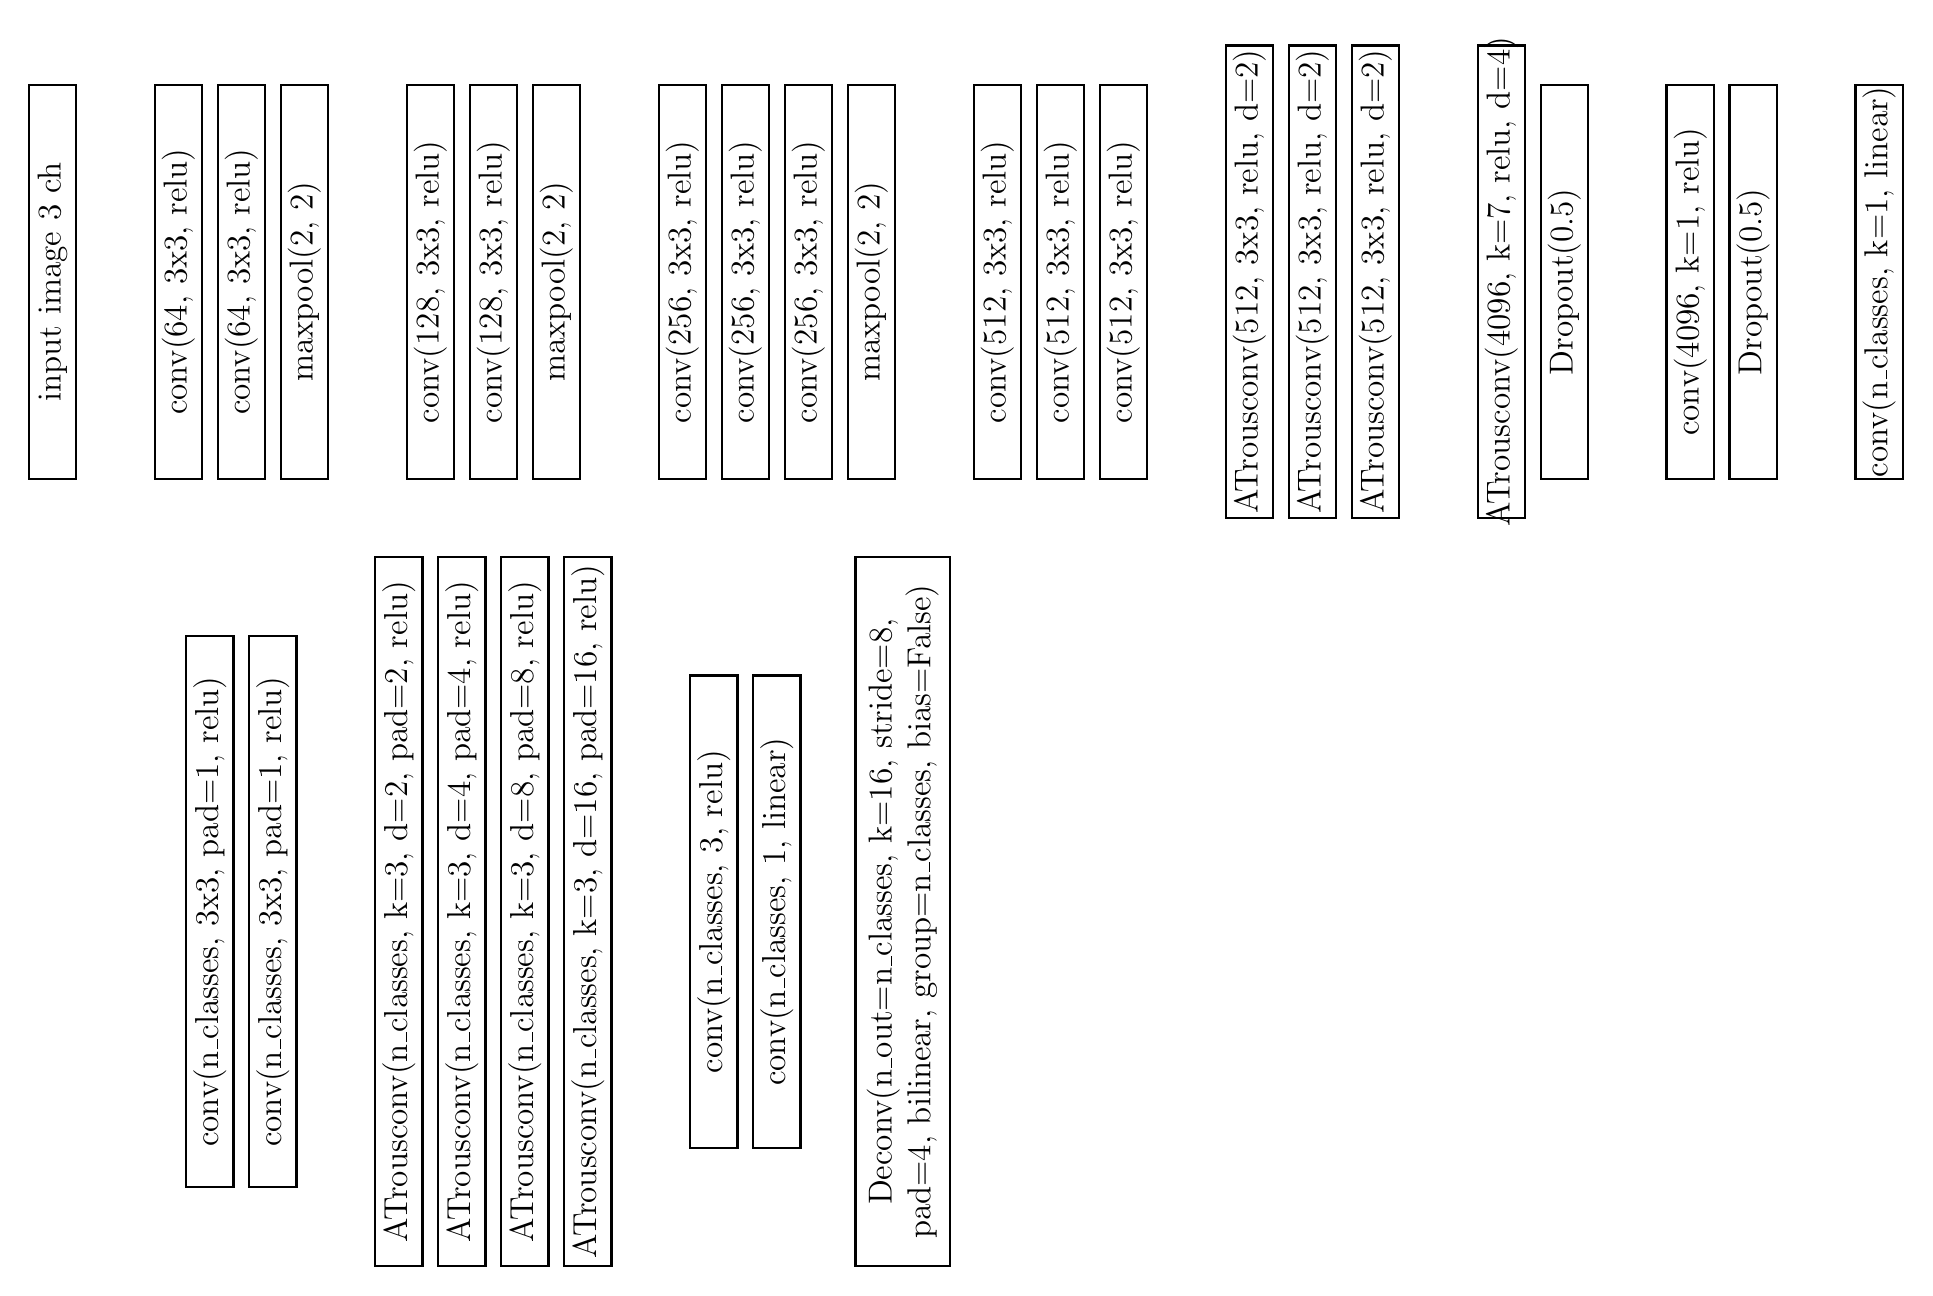
\begin{tikzpicture}

  \node (bx1) at (0,0) [draw,thick,minimum width=0.6cm,minimum height=5cm] {};
  \node[align=center,font=\large,rotate=90] at (bx1.center) {input image 3 ch};

  \node (bx21) at (1.6,0) [draw,thick,minimum width=0.6cm,minimum height=5cm] {};
  \node[align=center,font=\large,rotate=90] at (bx21.center) {conv(64, 3x3, relu)};
  \node (bx22) at (2.4,0) [draw,thick,minimum width=0.6cm,minimum height=5cm] {};
  \node[align=center,font=\large,rotate=90] at (bx22.center) {conv(64, 3x3, relu)};
  \node (bx23) at (3.2,0) [draw,thick,minimum width=0.6cm,minimum height=5cm] {};
  \node[align=center,font=\large,rotate=90] at (bx23.center) {maxpool(2, 2)};

  \node (bx31) at (4.8,0) [draw,thick,minimum width=0.6cm,minimum height=5cm] {};
  \node[align=center,font=\large,rotate=90] at (bx31.center) {conv(128, 3x3, relu)};
  \node (bx32) at (5.6,0) [draw,thick,minimum width=0.6cm,minimum height=5cm] {};
  \node[align=center,font=\large,rotate=90] at (bx32.center) {conv(128, 3x3, relu)};
  \node (bx33) at (6.4,0) [draw,thick,minimum width=0.6cm,minimum height=5cm] {};
  \node[align=center,font=\large,rotate=90] at (bx33.center) {maxpool(2, 2)};

  \node (bx41) at (8,0) [draw,thick,minimum width=0.6cm,minimum height=5cm] {};
  \node[align=center,font=\large,rotate=90] at (bx41.center) {conv(256, 3x3, relu)};
  \node (bx42) at (8.8,0) [draw,thick,minimum width=0.6cm,minimum height=5cm] {};
  \node[align=center,font=\large,rotate=90] at (bx42.center) {conv(256, 3x3, relu)};
  \node (bx43) at (9.6,0) [draw,thick,minimum width=0.6cm,minimum height=5cm] {};
  \node[align=center,font=\large,rotate=90] at (bx43.center) {conv(256, 3x3, relu)};
  \node (bx44) at (10.4,0) [draw,thick,minimum width=0.6cm,minimum height=5cm] {};
  \node[align=center,font=\large,rotate=90] at (bx44.center) {maxpool(2, 2)};

  \node (bx51) at (12,0) [draw,thick,minimum width=0.6cm,minimum height=5cm] {};
  \node[align=center,font=\large,rotate=90] at (bx51.center) {conv(512, 3x3, relu)};
  \node (bx52) at (12.8,0) [draw,thick,minimum width=0.6cm,minimum height=5cm] {};
  \node[align=center,font=\large,rotate=90] at (bx52.center) {conv(512, 3x3, relu)};
  \node (bx53) at (13.6,0) [draw,thick,minimum width=0.6cm,minimum height=5cm] {};
  \node[align=center,font=\large,rotate=90] at (bx53.center) {conv(512, 3x3, relu)};

  \node (bx61) at (15.2,0) [draw,thick,minimum width=0.6cm,minimum height=6cm] {};
  \node[align=center,font=\large,rotate=90] at (bx61.center) {ATrousconv(512, 3x3, relu, d=2)};
  \node (bx62) at (16,0) [draw,thick,minimum width=0.6cm,minimum height=6cm] {};
  \node[align=center,font=\large,rotate=90] at (bx62.center) {ATrousconv(512, 3x3, relu, d=2)};
  \node (bx63) at (16.8,0) [draw,thick,minimum width=0.6cm,minimum height=6cm] {};
  \node[align=center,font=\large,rotate=90] at (bx63.center) {ATrousconv(512, 3x3, relu, d=2)};

  \node (bx71) at (18.4,0) [draw,thick,minimum width=0.6cm,minimum height=6cm] {};
  \node[align=center,font=\large,rotate=90] at (bx71.center) {ATrousconv(4096, k=7, relu, d=4)};
  \node (bx72) at (19.2,0) [draw,thick,minimum width=0.6cm,minimum height=5cm] {};
  \node[align=center,font=\large,rotate=90] at (bx72.center) {Dropout(0.5)};

  \node (bx81) at (20.8,0) [draw,thick,minimum width=0.6cm,minimum height=5cm] {};
  \node[align=center,font=\large,rotate=90] at (bx81.center) {conv(4096, k=1, relu)};
  \node (bx82) at (21.6,0) [draw,thick,minimum width=0.6cm,minimum height=5cm] {};
  \node[align=center,font=\large,rotate=90] at (bx82.center) {Dropout(0.5)};

  \node (bx91) at (23.2, 0) [draw,thick,minimum width=0.6cm,minimum height=5cm] {};
  \node[align=center,font=\large,rotate=90] at (bx91.center) {conv(n\_classes, k=1, linear)};



  \node (bx101) at (2,-8) [draw,thick,minimum width=0.6cm,minimum height=7cm] {};
  \node[align=center,font=\large,rotate=90] at (bx101.center) {conv(n\_classes, 3x3, pad=1, relu)};
  \node (bx102) at (2.8,-8) [draw,thick,minimum width=0.6cm,minimum height=7cm] {};
  \node[align=center,font=\large,rotate=90] at (bx102.center) {conv(n\_classes, 3x3, pad=1, relu)};

  \node (bx111) at (4.4,-8) [draw,thick,minimum width=0.6cm,minimum height=9cm] {};
  \node[align=center,font=\large,rotate=90] at (bx111.center) {ATrousconv(n\_classes, k=3, d=2, pad=2, relu)};
  \node (bx112) at (5.2,-8) [draw,thick,minimum width=0.6cm,minimum height=9cm] {};
  \node[align=center,font=\large,rotate=90] at (bx112.center) {ATrousconv(n\_classes, k=3, d=4, pad=4, relu)};
  \node (bx113) at (6,-8) [draw,thick,minimum width=0.6cm,minimum height=9cm] {};
  \node[align=center,font=\large,rotate=90] at (bx113.center) {ATrousconv(n\_classes, k=3, d=8, pad=8, relu)};
  \node (bx114) at (6.8,-8) [draw,thick,minimum width=0.6cm,minimum height=9cm] {};
  \node[align=center,font=\large,rotate=90] at (bx114.center) {ATrousconv(n\_classes, k=3, d=16, pad=16, relu)};

  \node (bx121) at (8.4,-8) [draw,thick,minimum width=0.6cm,minimum height=6cm] {};
  \node[align=center,font=\large,rotate=90] at (bx121.center) {conv(n\_classes, 3, relu)};
  \node (bx122) at (9.2,-8) [draw,thick,minimum width=0.6cm,minimum height=6cm] {};
  \node[align=center,font=\large,rotate=90] at (bx122.center) {conv(n\_classes, 1, linear)};

  \node (bx131) at (10.8,-8) [draw,thick,minimum width=1.2cm,minimum height=9cm] {};
  \node[align=center,font=\large,rotate=90] at (bx131.center) {Deconv(n\_out=n\_classes, k=16, stride=8, \\pad=4, bilinear, group=n\_classes, bias=False)}; 
        \end{tikzpicture}
        \end{document}
